\section{Ausblick} % (fold)
\label{sec:ausblick}
	Sowohl für die Endanwender als auch für die Entwickler und Designer hat die Zukunft vor allem positive Änderungen parat. Das Http/1.1 Protokoll wird durch Http/2.0 abgelöst. Der LTE-Netzausbau schreitet weiter voran, deckt dabei eine immer größere Fläche ab und bringt den Nutzern damit eine niedrigere Latenz und eine höhere Bandbreite. Auf der diesjährigen Cebit wurde der neue Mobilfunkstandard \texttt{5G} von Vodafone präsentiert. Dieser steht noch in der Entwicklung, wird aber für das Jahr 2020 für den kommerziellen Einsatz vorhergesagt. 5G soll dabei Latenzen zwischen 1 bis 10 Millisekunden liefern und eine 100 mal höhere Bandbreite von bis zu 10.000 MBit/s zur Verfügung stellen.\autocite{lte-anbieter15} Ob diese Geschwindigkeiten auch wirklich innerhalb von nur 5 Jahren erreicht werden können, oder ob sie in erster Linie nur der \texttt{PR} dienen, bleibt dabei abzuwarten.

	\subsection{Http/2.0} % (fold)
	\label{sub:http_2_0}
		\begin{figure}[htbp]
			\begin{center}
				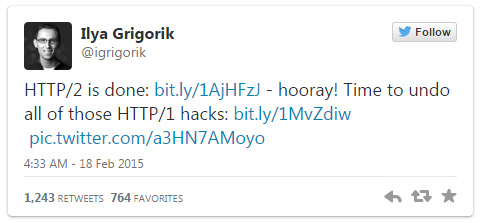
\includegraphics[width=0.5\textwidth]{http2_done.jpg}
				\caption{Http 2.0 wurde veröffentlicht}
				\label{fig:http2_done}
			\end{center}
		\end{figure}

		Dieses Jahr ist es soweit und das Http/1.1 Protokoll aus dem Jahre 1999 wird durch Http/2 abgelöst. Natürlich verschwindet das alte Protokoll nicht von heute auf morgen. Http/1.1 wird noch viele Jahre erhalten bleiben, vielleicht auch nie gänzlich verschwinden. Dennoch sagt Daniel Stenberg, Mitglieder der Http/2 Work Group, voraus, dass bis Ende 2015 der Anteil an Http/2 traffic mehr als 10\% beträgt \autocite{stenberg15}. Die großen Browser Chrome und Firefox haben in ihrer aktuellen Version Http/2 bereits aktiviert und auch der Internet Explorer soll mit Windows 10 (in der \texttt{Technical Preview} bereits aktiv) Http/2 unterstützen.\autocite{microsoft14} Schlusslicht bildet Apple mit seinem Safari Browser, von denen bis Dato (01.04.2015) noch keine Stellungnahme zu Http/2 verlautet wurde.
		Die zwei weitverbreitesten Server Apache und Nginx sind dabei, Http/2 zur Verfügung zu stellen. Apache hat bereits ein Http/2 Modul in der Alpha Phase. Nginx sagt, dass sie bis Ende 2015 Http/2 unterstützen werden.\\
		Google (damit auch Youtube und andere Produkte die zu Google gehören) und Twitter haben bereits Http/2 seit einigen Monaten aktiviert. Http/2 bietet folgende Performance Verbesserungen:

		\begin{itemize}
			\item Parallel Multiplexing anstatt der Verwendung von Parallelen Verbindungen
			\item Verwendet nur eine einzige TCP Verbindung
			\item Server-Push
		\end{itemize}
		
		\subsubsection{Http/1.1 Optimierungen in Http/2} % (fold)
		\label{ssub:http_1_1_optimierungen_in_http_2}
			Viele Optimierungs-Pattern für Http/1.1 stellen sich für das Http/2 Protokoll als Anti-Pattern heraus. Http/2 bringt den Vorteil, dass es genau eine TCP Verbindung benötigt. Damit wird \texttt{Domain Sharding} ein Performance Anti-Pattern für HTTP 2.0. Auch die Verwendung von \texttt{Image Sprites}, das Zusammenfügen von CSS und Javascript zu einer Datei ist ein Anti-Pattern wenn Http/2 verwendet wird. Eine Vielzahl von kleinen einzelnen Dateien werden zu keinem Performance Problem mehr durch Http/2.\autocite{grigorikHttp2}\\
			"`Server Push"' ist eine Mechanik die in Http/1.1 durch das Inlinen von CSS in das HTML Dokument bereits simuliert wird. De facto ist dies ein Workaround für eine Funktionalität die nun durch Http/2 bereitstellt wird. Durch Inlinen wird bei einer Anfrage gleich das CSS / Javascript als Antwort mitgesendet, das der Browser zur Darstellung des "`above the fold"' Inhaltes braucht.

			\begin{figure}[htbp]
				\begin{center}
					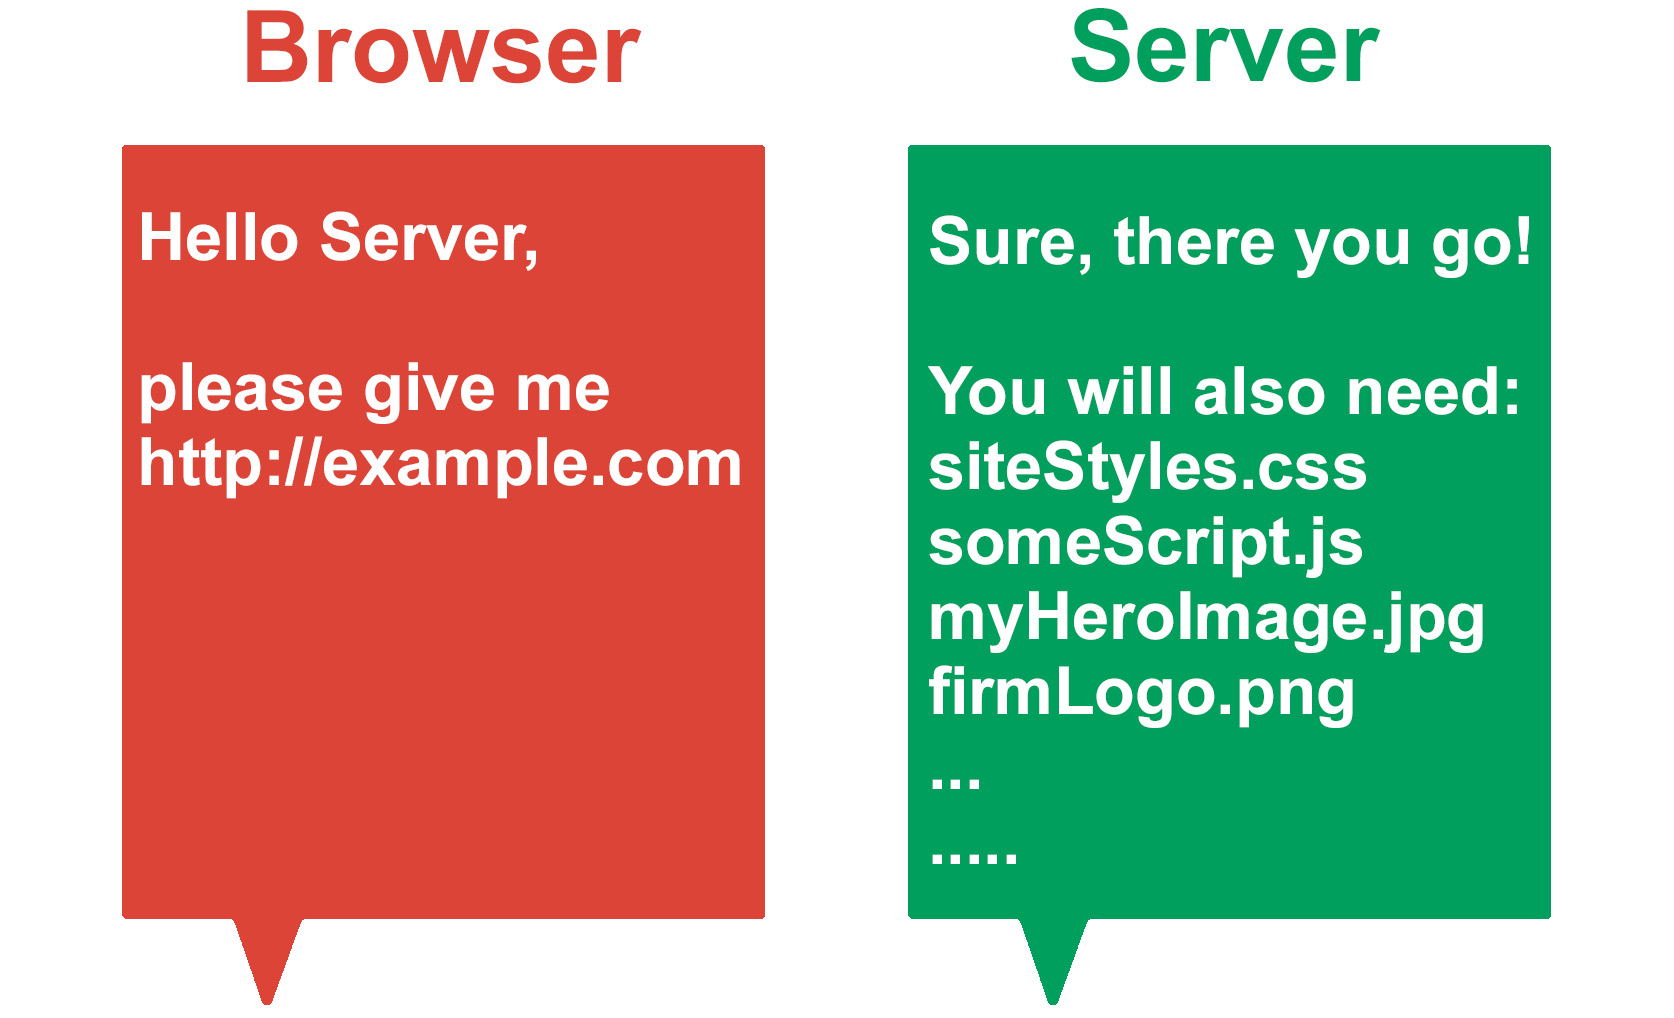
\includegraphics[width=0.6\textwidth]{server_push.jpg}
					\caption{Veranschaulichung der Server Push Mechanik (Eigene Abbildung)}
					\label{fig:server_push}
				\end{center}
			\end{figure}
			
			Durch \texttt{Server Push} wird genau dies möglich, ohne es inline in das Dokument zu schreiben. Dadurch sind die Ressourcen vom Browser im Cache speicherbar und können auch in den Unterseiten verwendet werden. Bereits bevor der Anwender die Seite besucht weiß man, welche Ressourcen ihm zur Verfügung gestellt werden müssen, um die Seite anzuzeigen. Diese Ressourcen lassen sich somit gleich auf die erste Anfrage als Antwort mitsenden und es wird damit das explizite \texttt{Anfragen und Antworten} eingespart.\footnote{Dieses Video stellt eindrücklich die Auswirkung der Server Push Mechanik vor (Länge 5 Minuten): \url{https://youtu.be/4Ai_rrhM8gA?t=29}}\\

			Durch Http/2 ergeben sich viele Vereinfachungen, aber auch neue Herausforderungen. Der Umstieg von Http/1.1 auf Http/2 wird nicht über Nacht geschehen. Für viele Seitenbetreiber wird es deshalb nötig sein, sowohl auf das alte, wie auch das neue Protokoll zu optimieren und an den jeweiligen Anwender die jeweils richtige Version auszuliefern. Dafür gibt es mehrere Ansätze und eine ausführliche Beschreibung gibt es hier: \url{http://tinyurl.com/phnq5d9}. \footnote{Eine detailierte Erklärung zu Http/2.0 ist dem PDF: http2 explained - Daniel Stenberg: \url{http://daniel.haxx.se/http2/http2-v1.11.pdf} zu entnehmen.}

		% subsubsection http_1_1_optimierungen_in_http_2 (end)

	% subsection http_2_0 (end)

\pagebreak
%
% section ausblick (end)
%


\section{Fazit} % (fold)
\label{sec:fazit}
	Web Performance ist ein wichtiges Thema und gewinnt weiterhin an Bedeutung. Dieses Projekt hat gezeigt, dass durch Analyse der eigenen Webanwendung und mittels Anwendung der \texttt{Best Practices} sehr schnelle Ladezeiten erzielt werden können. Es wurde auch erklärt, dass dies einen nicht unerheblichen Mehraufwand bedeutet, der nicht durch eine einzelne Person gestämmt werden kann, sondern sich innerhalb der gesamten Unternehmenskultur durchsetzen muss. Web Performance ist kein neues Thema, sondern wurde bereits sehr früh als eine Nummer Eins Priorität kommuniziert. Die Infrastruktur wird schneller, Browser werden weiterentwickelt und die Geräte werden leistungsstärker. Aber auch der Anwender wird dadurch immer verwöhnter und steigert seine Erwartungen an die Anwendung und gibt sich mit lägeren Wartezeiten nicht mehr zufrieden. Dies hat zur Folge, dass Web Performance nun auch für kleinere Seiten oder Produktanbieter ein wichtiger Aspekt wird, wenn das Angebot auch mittels Smartphone Akzeptanz finden soll. Es kann sich lohnen dem Anwender eine umfassende, schnelle Online-Erfahrung zu bieten. Auch Agenturen wie zum Beispiel Deep-Impact aus der Schweiz, springen auf den Zug der Web Performance auf und beginnen damit zu werben:

	\begin{quote}
		\textit{"`We value stability, security, \textbf{performance}, and flexibility. We also love new and shiny."'} \url{http://www.deep-impact.ch/en/} 
	\end{quote}

	Es ist nicht ein Opfer das erbracht werden muss um den Endanwender glücklich zu stellen, sondern kann auch eine Chance sein, als "`frist-mover"' den Trend zu erkennen und der Konkurrenz einen Schritt voraus zu sein.

% section fazit (end)
